\newpage
\section{Registrazione}

\label{Registrazione}
\begin{figure}[ht]
	\centering
	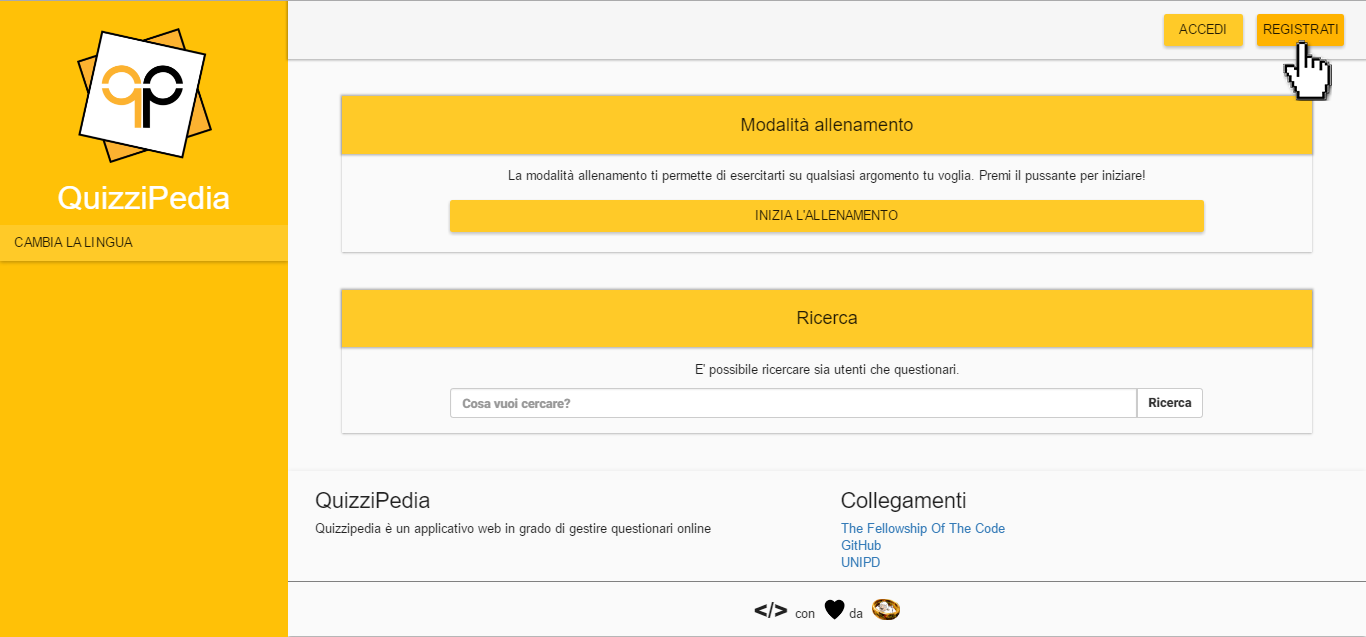
\includegraphics[scale=0.33]{img/vai_registrazione.png}
	\caption{Vai a Registrazione}
\end{figure}
\FloatBarrier

All'interno dell'Home Page è possibile accedere alla sezione \textit{Registrazione}. Una volta cliccato sul bottone apposito verrà presentata la seguente pagina:

\label{Registrazione_1}
\begin{figure}[ht]
	\centering
	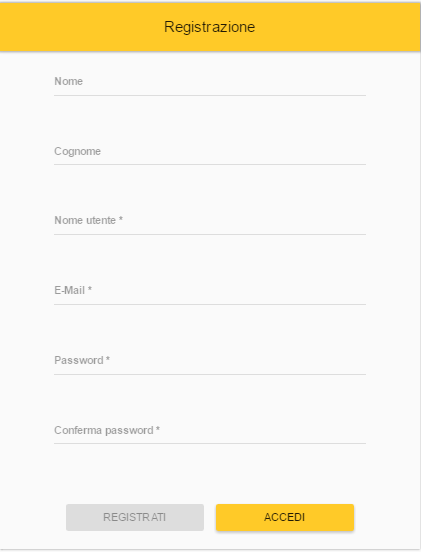
\includegraphics[scale=0.60]{img/registrazione.png}
	\caption{Registrazione}
\end{figure}
\FloatBarrier

L'utente per registrarsi deve obbligatoriamente compilare i seguenti campi:
\begin{itemize}
	\item Nome utente;
	\item E-mail;
	\item Password;
	\item Conferma password.
\end{itemize}
dove il campo \textit{Conferma password} deve essere identico al campo \textit{Password}, il quale deve avere almeno 8 caratteri. Compilati correttamente tutti i campi, il bottone \textit{Registrati}, prima disabilitato, permette di registrarsi effettuando un redirect alla pagina di autenticazione.  